%für Sprache, A4 Blatt, float, Grafiken, UTF Codierung, PDF, Color, Seitenabstand, Listings
\documentclass[a4papr,12pt]{article}
\usepackage[utf8]{inputenc}
\usepackage[ngerman]{babel}
\usepackage{graphicx}
\usepackage{float}
\usepackage{textcomp}
\usepackage{pdfpages}
\usepackage{tikz}
\usepackage{hyperref}
\usepackage{geometry}
\usepackage{listings}
\usepackage{color}

%Mathematics
\usepackage{amstext}
\usepackage{amssymb}
\usepackage{amsmath}
\usepackage{amsfonts}
\usepackage{mathrsfs}
\usepackage{mathtools}

%include this before fancy or page style gets messed up bc of geometry
%Seitenabstand A4 Blatt
\geometry{a4paper}
\geometry{top=25mm,bottom=25mm,left=23mm,right=20mm}

% macro to select a scaled-down version of Bera Mono (for instance)
\makeatletter
\newcommand\BeraMonottfamily{%
  \def\fvm@Scale{0.85}% scales the font down
  \fontfamily{fvm}\selectfont% selects the Bera Mono font
}
\makeatother

%Hyperref zum anklicken von Überschriften in Texmaker + Farben einstellen
\hypersetup{
	colorlinks,
	citecolor=black,
	filecolor=black,
	linkcolor=blue,
	urlcolor=black
}

\definecolor{mygreen}{rgb}{0,0.6,0}
\definecolor{mygray}{rgb}{0.5,0.5,0.5}
\definecolor{mymauve}{rgb}{0.58,0,0.82}

%Zum Pascal Code einfügen mit lstinputlisting[language=Pascal] {../blabla.pas}
\lstset{ %
  backgroundcolor=\color{white},   % choose the background color; you must add \usepackage{color} or 								  \usepackage{xcolor}
  basicstyle=\BeraMonottfamily,        % the size of the fonts that are used for the code
  breakatwhitespace=false,         % sets if automatic breaks should only happen at whitespace
  breaklines=true,                 % sets automatic line breaking
  captionpos=b,                    % sets the caption-position to bottom
  commentstyle=\color{mygreen},    % comment style
  deletekeywords={...},            % if you want to delete keywords from the given language
  escapeinside={\%*}{*)},          % if you want to add LaTeX within your code
  extendedchars=true,              % lets you use non-ASCII characters; for 8-bits encodings only, 												does not work with UTF-8
  frame=single,	               % adds a frame around the code
  keepspaces=true,                 % keeps spaces in text, useful for keeping indentation of code 									  (possibly needs columns=flexible)
  keywordstyle=\color{blue},       % keyword style
  language=Octave,                 % the language of the code
  otherkeywords={...},           % if you want to add more keywords to the set
  numbers=left,                    % where to put the line-numbers; possible values are (none, left, 								  right)
  numbersep=5pt,                   % how far the line-numbers are from the code
  numberstyle=\tiny\color{black}, % the style that is used for the line-numbers
  rulecolor=\color{black},         % if not set, the frame-color may be changed on line-breaks within 								  not-black text (e.g. comments (green here))
  showspaces=false,                % show spaces everywhere adding particular underscores; it 														overrides 'showstringspaces'
  showstringspaces=false,          % underline spaces within strings only
  showtabs=false,                  % show tabs within strings adding particular underscores
  stepnumber=2,                    % the step between two line-numbers. If it's 1, each line will be 								  numbered
  stringstyle=\color{mymauve},     % string literal style
  title=\getlstname,
  tabsize=2,	                    % sets default tabsize to 2 spaces
  inputencoding=latin1,
  columns=fullflexible
}

\lstset{literate=%
	{Ö}{{\"O}}1
	{Ä}{{\"A}}1
	{Ü}{{\"U}}1
	{ß}{{\ss}}1
	{ü}{{\"u}}1
	{ä}{{\"a}}1
	{ö}{{\"o}}1
	{~}{{\textasciitilde}}1
}

%Filenamen und Pfad trennen
\makeatletter
\DeclareRobustCommand{\getlstname}{%
\begingroup
  % \lstname seems to change hyphens into \textendash
  \def\textendash{-}%
  \filename@parse{\lstname}%
  \texttt{\filename@base.\filename@ext}%
\endgroup
}


%Für Kopfzeile den Style
\usepackage{fancyhdr}
\pagestyle{fancy}
\lhead{ADE - Übung 3}
\rhead{Andreas Roither, \today{}}
\newcommand{\Cross}{\mathbin{\tikz [x=1.4ex,y=1.4ex,line width=.2ex] \draw (0,0) -- (1,1) (0,1) -- (1,0);}}%

\begin{document}

%ANGABE 
\thispagestyle{plain}
\includepdf[pages={1},pagecommand={     
\begin{tikzpicture}[remember picture, overlay]\node at (15.8, -1.35) {4 h};\end{tikzpicture}
\begin{tikzpicture}[remember picture, overlay]\node at (7.6, -1.35) {Andreas Roither};\end{tikzpicture}
\begin{Huge}
\begin{tikzpicture}[remember picture, overlay]\node at (-1, -1.9) {X};\end{tikzpicture}
\end{Huge}
}]{Angabe/Uebung03.pdf}
%\includepdf[pages=2-,pagecommand={}]{testpdf}

\section*{Übung 3}
\subsection*{Aufgabe 1}
\subsubsection*{Lösungsidee}
Für das tauschen des Inhalts zweier Werte wird eine "`Zwischenspeicher Variable"' benötigt. Der Wert der ersten Variable wird zwischen gespeichert. Danach wird in der ersten Variable der Wert der zweiten Variable gespeichert. Anschließend wird mithilfe der Zwischenspeicher Variable der vorherige gespeicherte Wert von der zweiten Variable übernommen. Das funktioniert bei beiden Datentypen gleich, mit der Ausnahme das die Datentypen in der Prozedur und bei der Übergabe übereinstimmen müssen. 
\newline
\lstinputlisting[language=Pascal] {../swap.pas}
\begin{figure}[H]
	\centering
	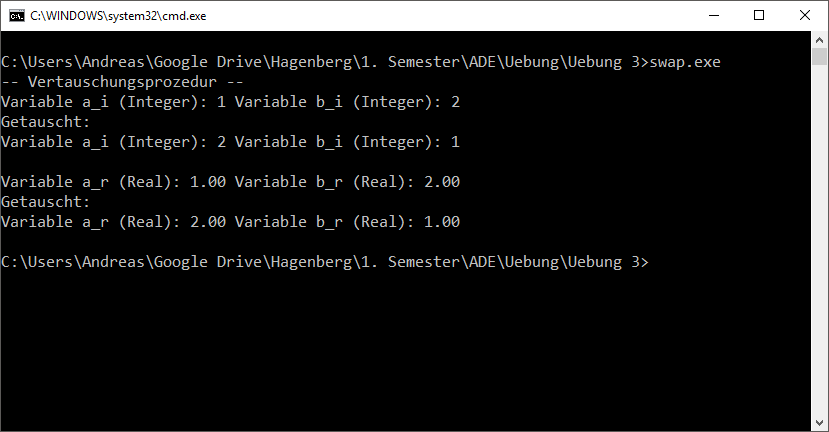
\includegraphics[scale=0.75]{./pictures/swap.png}
	\caption{Testfälle Vertauschungsprozedur}
	\label{fig: Spannweiten Berechnung}
\end{figure}

\section*{Testfälle}
Zum Testen werden vier Variablen mit zwei unterschiedlichen Datentypen initialisiert. Die Variablen mit gleichen Datentyp werden mit unterschiedlichen Werten versehen. Zum Testen werden die Variablen vor - und nach dem tauschen ausgegeben

\newpage

\subsection*{Aufgabe 2}
\subsubsection*{Lösungsidee}
Bei dem Konvertieren einer Dezimalzahl in eine Binärzahl wird folgendermaßen vorgegangen:
\begin{enumerate}
\item Die Zahl durch 2 dividieren
\item Der Rest der Division notieren
\item Falls das Ergebnis nicht 0 ist, Schritt 1 und 2 wiederholen
\item Die umgedrehte Reihenfolge des Restes nacheinander aufgeschrieben ergibt die Binärzahl
\end{enumerate}
Im Programm wird der Rest in $b_{0} .. b_{7}$ gespeichert und anschließend umgekehrt ($b_{7} .. b_{0}$) ausgegeben.
\newline
\lstinputlisting[language=Pascal] {../convert.pas}
\begin{figure}[H]
	\centering
	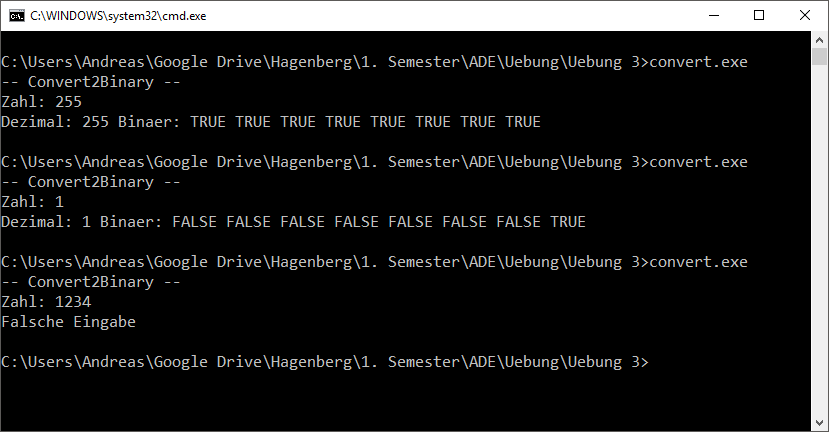
\includegraphics[scale=0.75]{./pictures/convert.png}
	\caption{Testfälle Zahlenkonvertierung}
	\label{fig: Sortieralgorithmus}
\end{figure}

\section*{Testfälle}
Zum Testen werden verschiedene Werte eingegeben, unter anderem auch ein zu hoher Wert.
\newpage

\subsection*{Aufgabe 3}
\subsubsection*{Lösungsidee}
Bei Max2 werden zwei Zahlen miteinander verglichen und das Maximum zurückgegeben. Max3a macht dasselbe mit drei Zahlen und gibt auch das Maximum zurück. Max3b macht sich den Rückgabewert der Max2 Funktion zunutze. Der Funktion werden die ersten beiden Input Zahlen von Max3b übergeben und das Resultat muss nur noch mit der übrigen letzen Input Zahl verglichen werden.
\newline
\lstinputlisting[language=Pascal] {../maxof2or3.pas}
\begin{figure}[H]
	\centering
	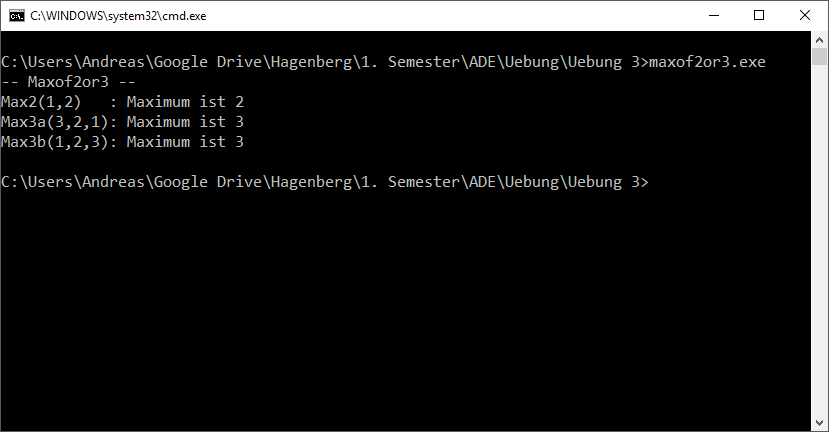
\includegraphics[scale=0.75]{./pictures/maxof2or3.png}
	\caption{Testfälle Maximum von zwei oder drei Zahlen}
	\label{fig: label}
\end{figure}

\section*{Testfälle}
Zum Testen werden Max2, Max3a und Max3b verschiedene Werte übergeben, auch in unterschiedlicher Reihenfolge.
\newpage

\subsection*{Aufgabe 4}
\subsubsection*{Lösungsidee}
Bei dieser Aufgabe muss eine Rundungsfunktion implementiert werden die sich printGraph zunutze macht. Falls das Ergebnis von (num mod 10) größer oder gleich 5 ist wird die zurückgegebene Zahl um eins erhöht. In der printGraph Funktion wird dann für jeweils die Positive und Negative Seite die Anzahl der X ausgegeben. Zusätzlich wird überprüft ob die Summe der Negativen und Positiven Seite nicht 100 überschreitet.
\newline
\lstinputlisting[language=Pascal] {../balkendiagramm.pas}
\begin{figure}[H]
	\centering
	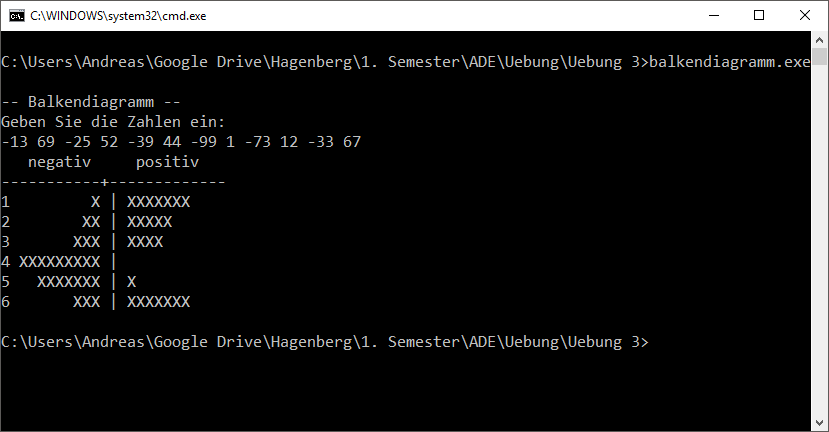
\includegraphics[scale=0.75]{./pictures/balkendiagramm.png}
	\caption{Testfall Balkendiagramm}
	\label{fig: label}
\end{figure}

\section*{Testfälle}
Zum Testen werden verschiedene Werte eingelesen, gerundet und anschließend die Zeilen mit der Anzahl von positiven und negativen X ausgegeben.

\newpage

\end{document}





